%%%%%%%%%%%%%%%%%%%%%%%%%%%%%%%%%%%%%%%%%%%%%%%
\chapter{Computational Results} \label{chap:comp_method}
%%%%%%%%%%%%%%%%%%%%%%%%%%%%%%%%%%%%%%%%%%%%%%%

In Table \ref{tab:r_over_t}, our vector solutions are computed by
Algorithm \ref{alg:Increasing-Method} for the $\left(\epsilon=1,\ell=1\right)-\ensuremath{N}_{3,r,4}$
network regarding to $t=2$ and $t=3$, with $q_{v}=q^{t}$ as previous
sections. Both construction 1 and 2 provide better results than scalar
solutions. 

Construction 1: $\begin{array}{c|c}
\boldsymbol{I}_{t} & \boldsymbol{T}\end{array}$, with $\boldsymbol{T}\in\ensuremath{\mathbb{F}}_{q}^{t\times t\left(h-1\right)}$

Construction 2: $\boldsymbol{T}\in MatrixSpaceUrs\left(t,3t\right)$

\section{Main Approach \label{sec:Main-Approach}}

Regarding to $t=2$, for a scalar network coding solution we need
a $3-\left(3,1,1\right)_{4}^{c}$ code ($q_{v}=2^{2}=4)$ by Theorem
\ref{theo:scalar_sol_exist}. The largest such code consists of the
21 one-dimensionall subspaces of $\ensuremath{\mathbb{F}}_{4}^{3}$,
each one is contained twice in the code. Therefore, the number of
nodes can be at most 42 for a scalar linear coding solution, while
for vector network coding 89 nodes can be used, i..e. $\mathcal{A}_{q=2}\left(n=6,k=4,\mathrm{t}=3;\lambda=2\right)\geq89$
following to Corollary \ref{cor:dual_subspaces}. This is a new lower
bound for $\mathcal{A}_{2}\left(6,4,3;2\right)$ compared to a code
with 51 codewords presented in \cite{Wachter-Zeh:2018}. The smallest
alphabet size for a scalar solution with 89 nodes exists is $q_{s}=8$.
By Equation \ref{eq:r_scalar_max}, there are 73 one-dimensional subspaces
of $\ensuremath{\mathbb{F}}_{8}^{3}$, and each one can be used twice
in the code; therefore, we have in total 146 possible codesword, but
only 89 codewords are required. In this case, the gap size $g=q_{s}-q_{v}=2^{3}-2^{2}=8-4=2^{2},$i.e.
we achieve a gap size $q^{t^{2}/2}$, which is better the asymptotic
behavior in \ref{eq:gap_e1l1h3rs4}. 

Before introducing the algorithm used to generate such 89 codewords,
we have to state some definitions for a beter explanation. We denote
a matrix space of dimension $\left[n\times m\right]$ by $M(n,m)=\left\{ \boldsymbol{A}:\boldsymbol{A}\in\ensuremath{\mathbb{F}}_{q=2}^{n\times m}\right\} $.
\begin{defn}[Matrix Space with Unique Row Space]
 $U(n,m)$ is a subset of $M(n,m)$, where any $\boldsymbol{A},\boldsymbol{B}\in U(n,m)$
have their row spaces such that:

\[
\mathcal{R}_{q}\left(\boldsymbol{A}\right)\neq\mathcal{R}_{q}\left(\boldsymbol{B}\right),
\]

where $\mathcal{R}_{q}\left(.\right)$ denotes the row space of a
matrix.
\end{defn}
%
\begin{defn}[Sufficient Global Coding Vector]
 Let $\boldsymbol{A},\boldsymbol{B},\boldsymbol{C}\in U(t,3t)$ and
$N\lll\left(\begin{array}{c}
2^{3t^{2}}\\
3
\end{array}\right)$, then a set $\mathcal{H}_{n=3t,m=3t}=\left\{ \boldsymbol{H}_{1},\ldots,\boldsymbol{H}_{N}\right\} $
contains distinct \textit{sufficient global coding vectors} $\boldsymbol{H}_{j}$
such that:

\[
rk\left[\boldsymbol{H}_{j}\right]=rk\left[\begin{array}{c}
\boldsymbol{A}\\
\boldsymbol{B}\\
\boldsymbol{C}
\end{array}\right]\geq2n,\forall j\in\left\{ 1,\ldots,N\right\} .
\]
\end{defn}
For ease of notations, we denote $\left[\begin{array}{c}
\boldsymbol{A}\\
\boldsymbol{B}\\
\boldsymbol{C}
\end{array}\right]$ by $\left\{ \boldsymbol{A},\boldsymbol{B},\boldsymbol{C}\right\} $
for the rest of this thesis.

\begin{defn}[Relative]
 Let $\boldsymbol{A},\boldsymbol{B},\boldsymbol{C}\in U(t,3t)$.
Then $\boldsymbol{C}$ is called a \textit{relative} of a tuple $\left(\boldsymbol{A},\boldsymbol{B}\right)$
if $\left\{ \boldsymbol{A},\boldsymbol{B},\boldsymbol{C}\right\} \in\mathcal{H}_{n=3t,m=3t}$
and denoted as following:

\[
rel\left[\left(\boldsymbol{A},\boldsymbol{B}\right)\right]=\boldsymbol{C}.
\]
\end{defn}
\begin{lem}
There are maximum $3\cdot\left(\begin{array}{c}
2^{3t^{2}}\\
3
\end{array}\right)$ relatives for a set $\mathcal{H}_{n=3t,m=3t}=\left\{ \boldsymbol{H}_{1},\ldots,\boldsymbol{H}_{N}\right\} $.
\label{lem:num_of_relatives}
\end{lem}
\begin{proof}
Each sufficient global coding vector $\boldsymbol{H}_{j}$ contains
a $\left\{ \boldsymbol{A},\boldsymbol{B},\boldsymbol{C}\right\} $.
Thus, each of these 3 matrices can form 3 different relatives:

\[
\begin{array}{c}
rel\left[\left(\boldsymbol{A},\boldsymbol{B}\right)\right]=\boldsymbol{C}\\
rel\left[\left(\boldsymbol{A},\boldsymbol{C}\right)\right]=\boldsymbol{B}\\
rel\left[\left(\boldsymbol{B},\boldsymbol{D}\right)\right]=\boldsymbol{A}
\end{array}.
\]

Furthermore, the maximum size of $\mathcal{H}_{n=3t,m=3t}$ is $q^{3t^{2}}$.
Therefore, $\mathcal{H}_{t=3}$ can have only maximum $3q^{3t^{2}}$
relatives.
\end{proof}
\begin{defn}[Sub-relative]
 Let $\boldsymbol{A},\boldsymbol{B},\boldsymbol{C},\boldsymbol{D}\in U(t,3t)$.
Then $\boldsymbol{D}$ is called a \textit{sub-relative} of a tuple
$\left(\boldsymbol{A},\boldsymbol{B},\boldsymbol{C}\right)\in\mathcal{H}_{n=3t,m=3t}$
if:

\[
\left\{ \begin{array}{c}
\left\{ \boldsymbol{A},\boldsymbol{B},\boldsymbol{D}\right\} \in\mathcal{H}_{t=3}\\
\left\{ \boldsymbol{A},\boldsymbol{C},\boldsymbol{D}\right\} \in\mathcal{H}_{t=3}\\
\left\{ \boldsymbol{B},\boldsymbol{C},\boldsymbol{D}\right\} \in\mathcal{H}_{t=3}
\end{array}\right..
\]

A sub-relative is denoted by: 
\[
subrel\left[\left(\boldsymbol{A},\boldsymbol{B},\boldsymbol{C}\right)\right]=\boldsymbol{D}
\]

This definition about Sub-relative is similarly again used for a set
of 5 or more matrices.
\end{defn}
\begin{algorithm}[H]
\caption{Increasing Method \label{alg:Increasing-Method}}

\hspace*{\algorithmicindent} \textbf{Input}: $\mathcal{H}_{n=3t,m=3t}$ with its size $\left|\mathcal{H}_{n=3t,m=3t}\right|=N\lll\left(\begin{array}{c} 2^{3t^{2}}\\ 3 \end{array}\right)$. \\
\hspace*{\algorithmicindent} \textbf{Output}: A $3-\left(3t,t,t\right)_{q=2}^{c}$ code or its orthogonal complement, a $3-\left(3t,2t,t\right)_{q=2}^{m}$ with its code size is maximum under $\mathcal{H}_{n=3t,m=3t}$.  
\begin{algorithmic}[1]
	\FORALL{$\left(\textbf{A},\textbf{B},\textbf{C}\right) \in \mathcal{H}_{n=3t,m=3t}$}
    	\STATE {$R\leftarrow$ Generate all relatives; ({*})}
	\ENDFOR

	\STATE {$P_{max}\leftarrow\{\}$ // an empty set}
	\FORALL{$\left(\textbf{X},\textbf{Y}\right) \in R$} 
		\IF{$\left|rel\left[\left(\textbf{X},\textbf{Y}\right)\right]\right|$ is maximum}
			\STATE {$P_{max}\leftarrow P_{max}\oplus\left(\textbf{X},\textbf{Y}\right)$ ({**})} 
		\ENDIF
	\ENDFOR

	\STATE {$P_{potential}\leftarrow\{\}$ // an empty set}
	\FORALL{$\left(\textbf{E},\textbf{Q}\right) \in P_{max}$}
		\IF{$\left|\left(\textbf{E},\textbf{Q}\right)\cup rel\left[\left(\textbf{E},\textbf{Q}\right)\right]\right|\notin P_{potential}$}
			\STATE {$P_{potential}\leftarrow P_{potential}\oplus\left(\textbf{E},\textbf{Q}\right)$}
		\ENDIF
	\ENDFOR
	
	\STATE {$P\leftarrow\{\}$ // an empty set}
	\FORALL{$\left(\textbf{K},\textbf{L}\right) \in P_{potential}$}
		\FORALL{$\textbf{Z} \in rel\left[\left(\textbf{X},\textbf{Y}\right)\right]$}
			\IF{$subrel\left[\left(\boldsymbol{K},\boldsymbol{L},\boldsymbol{Z}\right)\right]$ is maximum}
				\STATE {$P\leftarrow P_{potential}\oplus\left(\textbf{K},\textbf{L},\textbf{Z}\right)$ ({***})}
			\ENDIF
		\ENDFOR 
	\ENDFOR
	
	\WHILE{$\exists subrel$ in $P$ is not empty ({****})}
		\STATE {Line 10 to Line 23, but elements of $P_{max}$ is replaced by $P$ and the size of subrel or tuples are thus increased over each while loop.}
	\ENDWHILE
\end{algorithmic}
\end{algorithm}

({*}): If any 2-tuple exists already in $R$, its new relative is
appended to its existing relatives to form a set of relatives.

({*}{*}): $P_{max}$ is set to an empty set anytime we find a new
maximum, before the concatenation $\oplus$.

({*}{*}{*}): $P$ is set to an empty set anytime we find a new maximum,
before the concatenation $\oplus$. $P$ removes duplicated values
itself under the while-loop of Line 11 to Line 15.

({*}{*}{*}{*}): This means the maximum size of subrel in $P$ is not
0.

~

Now, we prove that Algorithm \ref{alg:Increasing-Method} always give
us our expected output. Then we compute its complexity based on number
of necessary computation.
\begin{proof}
Our problem can be described like finding all matrices such that any
3 of them can accompany together. The companion is possible, when
the 3 matrices satisfy the rank requirement in \ref{eq:rk_rqm_e1l1h3s4}.
The input $\mathcal{H}_{n=3t,m=3t}$ of Algorithm \ref{alg:Increasing-Method}
lists all such 3 matrices by tuples of 3 matrices (called 3-tuples).
Line 1 to Line 3 gives us all pairs or 2-tuples from these 3-tuples
as well as their relatives. Then the algorithm starts searching for
its output initially based on 2 matrices having the largest number
of relatives, i.e. it appears mostly in $\mathcal{H}_{n=3t,m=3t}$
in comparison with any other pairs of matrices. This number of relatives
plus 2 by themselves is actually the upper bound for a code size,
when a $3-\left(3t,t,t\right)_{q=2}^{c}$ code is considered \cite[Sec. V-D]{Zhang:2019}.
Furthermore, from Line 10 to Line 26, the algorithm extends the inital
2-tuples based on all of these relatives. That's why the algorithm's
output gives us all of our expected matrices.
\end{proof}
Our algorithm is based on $C_{relatives}\lll3\left(\begin{array}{c}
2^{3t^{2}}\\
3
\end{array}\right)\Rightarrow C_{relatives}\lll\mathcal{O}\left(\frac{t^{6}}{6}\right)$. In case $t=2$, $U(t,3t)$ helps us reduce $\left|M(t,3t)\right|=4096$
matrices to $\left|U(t,3t)\right|=715$ matrices, $C_{relatives}\approx3\left(\begin{array}{c}
\frac{715}{4096}2^{3t^{2}}\\
3
\end{array}\right)\approx\mathcal{O}\left(\frac{2}{3000}t^{6}\right)$. Therefore, we are able to achieve the output of Algorithm \ref{alg:Increasing-Method}
for $\mathcal{H}_{n=6,m=6}$ in a short amount of time.

We are going to list some toy examples for the algorithm as well as
illustrate it in Figure \ref{fig:rel_example}.
\begin{example}
Let $n=1,m=2,q=2$, which violates the input $\mathcal{H}_{n=3t,m=3t}$
but still being a good example for the rest steps in Algorithm \ref{alg:Increasing-Method}.
Then we have $N=4$ matrices (vectors):
\[
\begin{array}{c}
\boldsymbol{A}=[0,0]\\
\boldsymbol{B}=[0,1]\\
\boldsymbol{C}=[1,0]\\
\boldsymbol{D}=[1,1]
\end{array}
\]

\uline{Step 1} (Line 1 to Line 3): Due to, any 3 of them form a
sufficient global coding vector, i.e. a matrix with $rk\geq2n$, we
have the relative as following:
\[
\begin{array}{c}
rel\left[\left(\boldsymbol{A},\boldsymbol{B}\right)\right]=[\boldsymbol{C},\boldsymbol{D}]\\
rel\left[\left(\boldsymbol{A},\boldsymbol{C}\right)\right]=[\boldsymbol{B},\boldsymbol{D}]\\
rel\left[\left(\boldsymbol{A},\boldsymbol{D}\right)\right]=[\boldsymbol{B},\boldsymbol{C}]\\
rel\left[\left(\boldsymbol{B},\boldsymbol{C}\right)\right]=[\boldsymbol{A},\boldsymbol{D}]\\
rel\left[\left(\boldsymbol{B},\boldsymbol{D}\right)\right]=[\boldsymbol{A},\boldsymbol{C}]\\
rel\left[\left(\boldsymbol{C},\boldsymbol{D}\right)\right]=[\boldsymbol{A},\boldsymbol{B}]
\end{array}
\]

\uline{Step 2} (Line 4 to Line 9): We get the maximum size of these
steps is $2$ and $P_{max}$ results in all $\left\{ \boldsymbol{A},\boldsymbol{B}\right\} ,\left\{ \boldsymbol{A},\boldsymbol{C}\right\} ,\left\{ \boldsymbol{A},\boldsymbol{D}\right\} ,\left\{ \boldsymbol{B},\boldsymbol{C}\right\} ,\left\{ \boldsymbol{B},\boldsymbol{D}\right\} ,\left\{ \boldsymbol{C},\boldsymbol{D}\right\} $,
because $\underset{\begin{array}{c}
\forall\boldsymbol{X},\boldsymbol{Y}\in M(1,2)\\
\boldsymbol{X}\neq\boldsymbol{Y}
\end{array}}{max}\left(rel\left[\left(\boldsymbol{X},\boldsymbol{Y}\right)\right]\right)=2$.

\uline{Step 3} (Line 10 to Line 14): Due to $\left\{ \boldsymbol{E},\boldsymbol{Q}\right\} \cup rel\left[\left(\boldsymbol{E},\boldsymbol{Q}\right)\right]=\left\{ \boldsymbol{A},\boldsymbol{B},\boldsymbol{C},\boldsymbol{D}\right\} $
with $\left(\boldsymbol{E},\boldsymbol{Q}\right)$ are tuples from
$P_{max}$ found in Step 2. We keep only $P_{potential}=\left\{ \left(\boldsymbol{A},\boldsymbol{B}\right):rel\left[\left(\boldsymbol{A},\boldsymbol{B}\right)\right]\right\} $

\uline{Step 4} (Line 16 to 23): Regarding to $rel\left[\left(\boldsymbol{K},\boldsymbol{L}\right)\right]=rel\left[\left(\boldsymbol{A},\boldsymbol{B}\right)\right]$,
we have $\boldsymbol{Z}\in\left\{ \boldsymbol{C},\boldsymbol{D}\right\} $.
Then, $\left|subrel\left[\left(\boldsymbol{A},\boldsymbol{B},\boldsymbol{C}\right)\right]\right|=\left|subrel\left[\left(\boldsymbol{A},\boldsymbol{B},\boldsymbol{D}\right)\right]\right|=1$,
so we get $P=\left\{ \left(\boldsymbol{A},\boldsymbol{B},\boldsymbol{C}\right),\left(\left(\boldsymbol{A},\boldsymbol{B},\boldsymbol{D}\right)\right)\right\} $.

\uline{Step 5}: The maximum size of subrel in $P$ is larger than
$0$, so we proceed the while loop. Step 3 will be looped firstly,
and we get $P_{potential}=\left\{ \left(\boldsymbol{A},\boldsymbol{B},\boldsymbol{C}\right):rel\left[\left(\boldsymbol{A},\boldsymbol{B},\boldsymbol{C}\right)\right]\right\} $.

\uline{Step 6}: As step 4, we get a result $\left\{ \boldsymbol{A},\boldsymbol{B},\boldsymbol{C},\boldsymbol{D}\right\} $.
\end{example}
%
\begin{example}
For further understading, we use Figure \ref{fig:rel_example} for
illustration. In the right, we observe that the size of relative becomes
smaller when its tuple identity is larger, i.e. $\left|rel\left[\left(\boldsymbol{A},\boldsymbol{B}\right)\right]\right|\geq\left|subrel\left[\left(\boldsymbol{A},\boldsymbol{B},\boldsymbol{C}\right)\right]\right|$
or $\left|rel\left[\left(\boldsymbol{A},\boldsymbol{B}\right)\right]\right|\geq\left|subrel\left[\left(\boldsymbol{A},\boldsymbol{B},\boldsymbol{D}\right)\right]\right|$.
It explains why the maximum numbers of matrices that we can find for
a vector solution of this network is the output of Algorithm \ref{alg:Increasing-Method}.
Regarding to the left, the visual explanation of $subrel$ is shown.
\end{example}
\begin{figure}[H]
\caption{The vector network coding of $(\epsilon=1,l=1)-\mathcal{N}_{h=3,r,s=4}$
represents as a matrix problem\label{fig:rel_example}}

\centering{}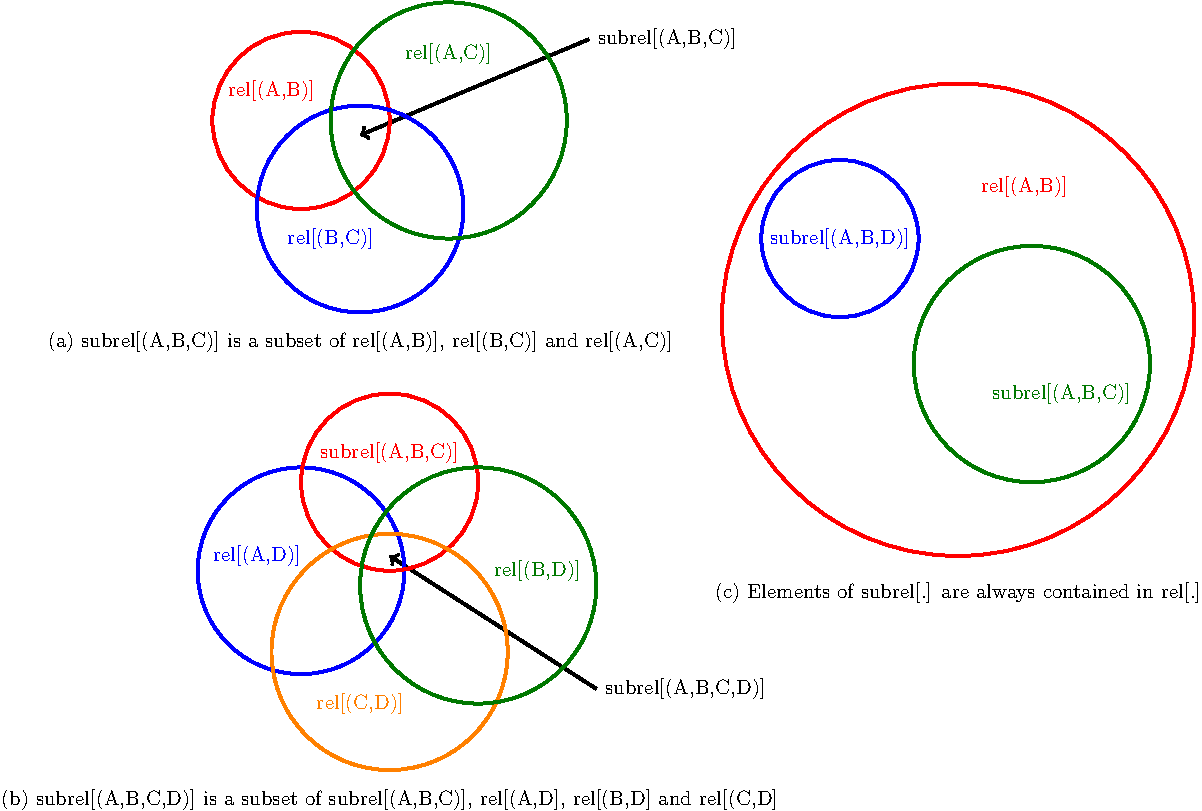
\includegraphics[width=0.5\paperwidth]{E:/Documents/TUM/THESIS/thesisCOD_Ha/figures/rel_example}
\end{figure}


\section{Alternative Approaches}

Firstly, instead of using \textit{matrix space with unique row space},
we use the whole matrix space $M\left(n,m\right)$. In case $t=2$,
we cover all $2^{3t^{2}}=4096$ matrices instead of only 715 matrices
in Section \ref{sec:Main-Approach}, which will help the Algorithm
\ref{alg:Increasing-Method} cover the optimal vector solution.
\begin{defn}[Good Global Coding Vector\label{def:almost_sufficient_global_coding_vector}]
 Let $\boldsymbol{A},\boldsymbol{B},\boldsymbol{C}\in U(t,3t)$ and
$N\leq\left(\begin{array}{c}
2^{3t^{2}}\\
3
\end{array}\right)$, then a set $\mathcal{T}_{n=3t,m=3t}=\left\{ \boldsymbol{T}_{1},\ldots,\boldsymbol{T}_{N}\right\} $
contains distinct \textit{sufficient global coding vectors} $\boldsymbol{T}_{j}$
such that:

\[
rk\left[\boldsymbol{T}_{j}\right]=rk\left[\begin{array}{c}
\boldsymbol{A}\\
\boldsymbol{B}\\
\boldsymbol{C}
\end{array}\right]\geq2n,\forall j\in\left\{ 1,\ldots,N\right\} .
\]
\end{defn}
In Algorithm \ref{alg:Increasing-Method}, we substitute the input
by $\mathcal{T}_{n=3t,m=3t}$ instead of $\mathcal{H}_{n=3t,m=3t}$.
This will give us an output with upper bound of $\mathcal{A}_{2}\left(3t,2t,3;2t\right)=126$
\cite[Sec. V-B]{Zhang:2019}.

Secondly, we tried another approach called ``Randomly Increasing
Method''. We got about 72 codewords instead of 89 codewords as Algorithm
\ref{alg:Increasing-Method}, due to a limited number of tries.

Finally, we tried removing bad matrices from a set of all 4096 matrices,
until any 3 of the matrices left in the set satisfy the Equation \ref{eq:rk_rqm_e1l1h3s4}.
A matrix with the less number of existence in $\mathcal{T}_{n=3t,m=3t}$
or $\mathcal{H}_{n=3t,m=3t}$ is evaluated as a bad matrix, and it
is removed for each step. If many bad matrices exist, we only remove
the first one. In case $t=2$, we unfortunately got about 69 codewords
instead of 89 codewords as Algorithm \ref{alg:Increasing-Method}.

\clearpage